\section{Pseudo-hiperparámetro \emph{nInputs}} \label{anexo:hyperNInputs}

El pseudo-hiperparámetro \emph{nInputs} se denomina de este modo debido a que su valor no puede ajustarse directamente, sino que queda determinado por la combinación de los tres hiperparámetros \emph{player}, \emph{pokemon} y \emph{move}, es un hiperparámetro combinado. Este parámetro representa el número de variables de entrada empleadas en la representación del estado. La distribución de los experimentos realizados en función de (\emph{nInputs}) se muestra en la figura \ref{fig:experimentsByNInputs} y la tabla \ref{tab:experimentsByNInputs}. Se observa que la representación compuesta por 182 variables de entrada es la más utilizada, mientras que el resto de configuraciones presentan una distribución uniforme.

\begin{table}[h]
    \centering
    {\small
        \begin{tabular}{lr}
            \toprule
            Número de parámetros & Número de experimentos \\
            \midrule
            182                  & 26                     \\
            1382                 & 5                      \\
            1898                 & 1                      \\
            1946                 & 1                      \\
            1982                 & 1                      \\
            2006                 & 1                      \\
            2066                 & 1                      \\
            2438                 & 8                      \\
            2546                 & 1                      \\
            2774                 & 5                      \\
            2834                 & 1                      \\
            2858                 & 2                      \\
            3206                 & 6                      \\
            3710                 & 1                      \\
            3724                 & 1                      \\
            3772                 & 2                      \\
            3782                 & 1                      \\
            3808                 & 3                      \\
            3832                 & 2                      \\
            3892                 & 2                      \\
            3986                 & 1                      \\
            4082                 & 1                      \\
            4346                 & 1                      \\
            4372                 & 3                      \\
            4394                 & 1                      \\
            4430                 & 1                      \\
            4454                 & 5                      \\
            4514                 & 1                      \\
            4684                 & 3                      \\
            4994                 & 1                      \\
            5044                 & 1                      \\
            5306                 & 1                      \\
            5536                 & 2                      \\
            5812                 & 2                      \\
            5908                 & 4                      \\
            6158                 & 3                      \\
            6434                 & 1                      \\
            6484                 & 2                      \\
            6530                 & 2                      \\
            7574                 & 4                      \\
            7634                 & 5                      \\
            9110                 & 6                      \\
            9328                 & 1                      \\
            14186                & 1                      \\
            16012                & 4                      \\
            16634                & 1                      \\
            30122                & 1                      \\
            31948                & 2                      \\
            32570                & 1                      \\
            37276                & 10                     \\
            54710                & 7                      \\
            82826                & 1                      \\
            \bottomrule
        \end{tabular}
    }
    \caption{Número de experimentos por representación del estado}
    \label{tab:experimentsByNInputs}
\end{table}

\begin{figure}[h]
    \centering
    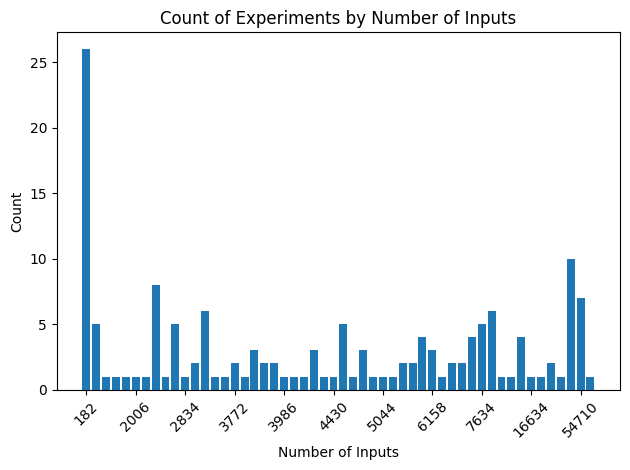
\includegraphics[width=0.8\textwidth]{images/ExperimentsByNInputs.png}
    \caption{Número de experimentos por representación del estado}
    \label{fig:experimentsByNInputs}
\end{figure}
